\documentclass[a4paper,12pt,Times]{article}
\usepackage{abakos}  %pacote com padrão da Abakos baseado no padrão da PUC

%%%%%%%%%%%%%%%%%%%%%%%%%%%
%Capa da revista
%%%%%%%%%%%%%%%%%%%%%%%%%%

%\setcounter{page}{80} %iniciar contador de pagina de valor especificado
\newcommand{\monog}{Revista Abakós do Instituto de Ciências Exatas e de Informática Pontifícia Universidade Católica de Minas Gerais}
\newcommand{\monogES}{Model - Magazine Abakós - ICEI - PUC Minas}
\newcommand{\tipo}{Artigo }  % Especificar a seção tipo do trabalho: Artigo, Resumo, Tese, Dociê etc
\newcommand{\origem}{Brasil}
\newcommand{\editorial}{\textbf{Abakos}, Belo Horizonte,v. 1, n. 1, p. 00-00, Jul. 2013 - ISSN: 2316-9451}  % p. xx-xx – páginas inicial-final do artigo
% \newcommand{\lcc}{\scriptsize{Licença Creative Commons Attribution-NonCommercial-NoDerivs 3.0 Unported}}

%%%%%%%%%%%%%%%%%INFORMAÇÕES SOBRE AUTOR PRINCIPAL %%%%%%%%%%%%%%%%%%%%%%%%%%%%%%%
\newcommand{\AutorA}{Renato Weverton Oliveira de Assis}
\newcommand{\funcaoA}{}
\newcommand{\emailA}{renatoweverton@gmail.com}
\newcommand{\cursA}{Bacharel em Sistemas de Informação PUC Minas}
% 
% \newcommand{\AutorB}{Fernando José Rodrigues Cordeiro}
% \newcommand{\funcaoB}{Bacharel em Sistemas de Informação}
% \newcommand{\emailB}{fernandocordeiro@pucminas.br}
% \newcommand{\cursB}{Instituto de Ciências Exatas e de Informática da PUC Minas}
% 
% \newcommand{\AutorC}{Giovanni Candido da Silva}
% \newcommand{\funcaoC}{Bacharel em Sistemas de Informação}
% \newcommand{\emailC}{giovanni@pucminas.br}
% \newcommand{\cursC}{Instituto de Ciências Exatas e de Informática da PUC Minas}

% Definir macros para o nome da Instituição, da Faculdade, etc.
\newcommand{\univ}{Pontifícia Universidade Católica de Minas Gerais}

\newcommand{\keyword}[1]{\textsf{#1}}

\begin{document}
% %%%%%%%%%%%%%%%%%%%%%%%%%%%%%%%%%%
% %% Pagina de titulo
% %%%%%%%%%%%%%%%%%%%%%%%%%%%%%%%%%%

\begin{flushleft}

\begin{minipage} [c][5cm][b]{16.5cm} % a primeira minipágina tem uma altura de 1.5cm e uma largura de 2.3cm.
% comando que introduz o logo da escola que nesta altura já terá de estar na pasta imagens que 
%por sua vez está na pasta onde se guardou o arquivo tex. E introduzimos essa imagem com a mesma altura da minipage.

\includegraphics[scale=1.1]{figuras/pucmg.png} 
\end{minipage}

 \vspace{0cm} {
 \singlespacing \Large{\monog \symbolfootnote[1]{Artigo apresentado à Revista Abakos} \\ }
  \normalsize{\monogES}
 }
\end{flushleft}
\begin{flushright}
\singlespacing 
\normalsize{\AutorA \footnote{\funcaoA \cursA, \origem -- \emailA }} \\
% \normalsize{\AutorB \footnote{\funcaoB, E-mail:\emailB \\ \cursB, \origem. }} \\
% \normalsize{\AutorC \footnote{\funcaoC, E-mail:\emailC \\ \cursC, \origem. }} \\
% \normalsize{\AutorD \footnote{\funcaoD \\ Pais de origem: \origemD. E-mail: \emailD}} \\
%deixar com o valor `0` e usar o '*' no inicio da frase
% \symbolfootnote[0]{Artigo recebido em 10 de julho de 1983 e aprovado em 29 de maio 2012}
\end{flushright}
\thispagestyle{empty}

\begin{abstract}
\noindent
	Ferramentas de gerenciamento de configuração, são basicamente framework para a construção de ambientes computacionais, permitindo a implantação e gestão de sistemas de informação em servidores. Essa construção é dada por meio de linguagens declarativas, através de instruções para a construção de cenários e suas respectivas configurações e regras.
    Este trabalho trata-se da avaliação de ferramentas de gerenciamento de configuração, destacando-se pelas características: vantagens, desvantagens, complexidade de configuração, popularidade entre os usuários, suporte, preço, documentação, plataformas suportadas e demonstração básica de funcionamento dessas.
\\\textbf{\keyword{Palavras-chave: }} Template. \LaTeX. Abakos. Periódicos.
\end{abstract}

%%%%%%%%%%%%%%%%%%%%%%%%%%%%%%%%%%%%%%%%%%%%%%%%%%%%%%%%%
\newpage 
\selectlanguage{english}
\begin{abstract}
\noindent
The abstract should contain at least one hundred and fifty words in accordance with the standards of ABNT standard.
This present article will address the main features of the web programming languages, that are used currently, 
comparing its features as to indicate to indicate the better use of determined language. 
The linguage will be divided according with four major caracteristics: Interpreted, compiled, server-side and client-side.
This present article will address the main features of the web programming languages.
The abstract should contain at least one hundred and fifty words in accordance with the standards of ABNT standard.
The linguage will be divided according with four major caracteristics: Interpreted, compiled, server-side and client-side.
This present article will address the main features of the web programming languages.
The abstract should contain at least one hundred and fifty words in accordance with the standards of ABNT standard.
\\\textbf{\keyword{Keywords: }} Template. \LaTeX. Abakos. Periodics.
\end{abstract}

\selectlanguage{brazilian}
 \onehalfspace  % espaçamento 1.5 entre linhas
 \setlength{\parindent}{1.25cm}

%%%%%%%%%%%%%%%%%%%%%%%%%%%%%%%%%%%%%%%%%%%%%%%%%
%% INICIO DO TEXTO
%%%%%%%%%%%%%%%%%%%%%%%%%%%%%%%%%%%%%%%%%%%%%%%%%

%%%%%%%%%%%%%%%%%%%%%%%%%%%%%%%%%%%%%%%%%%%%%%%%%%%%%%%%%%%%%%%%%%%%%%%%%%%%%%%%%%%%%%%%%%%%%%%%%%%%%%%
%%%%%%%%%%%%%% Template de Artigo Adaptado para Trabalho de Diplomação do ICEI %%%%%%%%%%%%%%%%%%%%%%%%
%% codificação UTF-8 - Abntex - Latex -  							     %%
%% Autor:    Fábio Leandro Rodrigues Cordeiro  (fabioleandro@pucminas.br)                            %% 
%% Co-autor: Prof. João Paulo Domingos Silva  e Harison da Silva                                     %%
%% Revisores normas NBR (Padrão PUC Minas): Helenice Rego Cunha e Prof. Theldo Cruz                  %%
%% Versão: 1.0     13 de março 2014                                                                  %%
%%%%%%%%%%%%%%%%%%%%%%%%%%%%%%%%%%%%%%%%%%%%%%%%%%%%%%%%%%%%%%%%%%%%%%%%%%%%%%%%%%%%%%%%%%%%%%%%%%%%%%%
\chapter{INTRODUÇÃO}

Em um mercado globalizado e competitivo, as tecnologias da informação se tornaram fundamentais para o auxílio da gestão das empresas em suas atividades rotineiras e também no suporte a tomadas de decisões e a possibilidade de desenvolvimento de novos negócios, novos modelos de negócio e a modificação dos valores estratégicos das empresas. \cite{audy}.

Visando a adequação as mudanças mercadológicas, organizacionais e a manutenibilidade em relação a concorrência, o investimento em sistemas de informação tem uma grande parcela do orçamento das empresas, buscando o alinhando da Tecnologia da informação e negócios. \cite{luftman}  
Para a atender essas necessidades, os requisitos de sistemas têm se tornado cada vez mais complexos, voláteis e robustos diante as demandas das organizações. 
As denominadas metodologias ágeis permitem a entrega de software funcionais em ciclos desenvolvimento mais curtos considerando a velocidade demandada para a sua construção. \cite{sbbrocco} 
          
No entanto as equipes que lidam com a infraestrutura têm a difícil tarefa de implantar um software em produção a medida em que são criados ou modificados, pois estes sistemas requerem dependências de componentes externos, como configurações de hardware, sistemas operacionais, banco de dados, servidores de aplicação e web e ainda configurações especificas da aplicação. Isto demanda um tempo considerável para a implantação destes sistemas.

Para garantir um processo totalmente ágil, que acompanhe as exigências do negócio da organização é necessário que haja uma integração do desenvolvimento de sistemas e as operações de infraestrutura. Portanto essa abordagem ágil também deve ser seguida pelas equipes de infraestrutura.
O movimento cultural denominado DevOps surgido em meado de 2009, influenciado principalmente por metodologias ágeis e computação na nuvem. Tem como fundamento a automatização de processos das operações de infraestrutura e a integração entre as equipes de desenvolvimento e operações. \cite{sato}.

\section{\esp Contextualização}
A automatização de processos de infraestrutura é uma das premissas do DevOps, utilizando uma abordagem para gerenciar servidores e seus recursos, tais como, máquinas virtuais, armazenamento, segurança e redes, destinando-se a simplificar significativamente a configuração e o gerenciamento de recursos em pequena e grande escala. A tradicional administração de um data center ou uma nuvem exige que a cada alteração de software, uma eventual ação manual na infraestrutura para acetar as configurações. Com a automação a infraestrutura também é tratada como "código" e um desenvolvedor pode escrever os recursos exigidos por uma aplicação em um arquivo padronizado e software de provisionamento se encarrega lê-lo e criar,atualizar ou deletar os recursos mantendo o estado atual da infraestrutura. 


\section{\esp Justificativa}
A justificativa deste trabalho é a oportunidade de aprendizado de tecnologias voltadas para o provisionamento de infraestrutura como código de ambientes de computacionais, nuvem ou físico.  

\section{\esp Objetivos}
\subsection{\esp Objetivo Geral}

Realizar um ensaio comparativo entre dois softwares de provisionamento de infraestrutura \textbf{Ansible} e \textbf{Chef}.

\subsection{\esp Objetivos Específicos}
\begin{itemize}
\item Apresenta um conceito básico de DevOps e suas práticas e os conceitos de infraestrutura como código.
\item Apresentar os principais conceitos chaves de cada ferramenta.
\item Apresentar os principais componentes de cada ferramenta.
\item Apresentar os critérios avaliativos e  métricas
\item Demonstrar o funcionamento das ferramentas.
\item Apresentar um comparativo e os resultados e as conclusões 
\end{itemize}
\section{\esp ESTRUTURA DO TRABALHO}
Este trabalho é composto por uma introdução, contextualização, justificativas e objetivos e os seguintes capítulos:
\begin{itemize}
\item Capitulo 2 - Revisão literária: traz  o referencial teórico apresentando um conceito básico de DevOps e práticas e os conceitos de infraestrutura como código.  
\item Capitulo 3 - Apresenta os principais conceitos chaves e características de cada ferramenta
\item Capitulo 4 - Apresenta os principais componentes de cada ferramenta.
\item Capítulo 5 - Apresenta os critérios avaliativos e  métricas
\item Capítulo 6 - Funcionamento básico: Demonstra o funcionamento das ferramentas 
\item Capítulo 7 - Comparativo entre as ferramentas: Apresenta as os resultados e conclusões
\end{itemize}

\chapter{ Revisão literária}

Este capítulo apresenta uma revisão da literatura sobre as definições de \textit{DevOps}, e os conceitos de infraestrutura como código e as suas principais características e práticas e fatores que envolvam sua adoção. 


O que é DevOps?

        O movimento Ágil tem como premissas a comunicação, colaboração e interações, 
formando equipes altamente eficazes multidisciplinares que compartilham os mesmos objetivos. ou seja, focam em indivíduos e entrega de software e não em processos. 
Os membros das equipes compreendem as funções e papeis de todos, permitindo que 
uma equipe de programadores e testadores trabalhem em sintonia. Isso proporcionam 
que as equipes desempenharem seu principal papel que é o desenvolvimento do produto.   \cite{sbbrocco}

    Entregar software em produção é um processo que tem se tornado cada vez
mais complexo em diversas empresas. Ciclos longos de desenvolvimento,
teste e a implatação do sistema em produçãoo alguns
dos fatores que contribuem para este problema. Mesmo equipes ágeis que
produzem software incremental ao final de cada iteração. O software para ser implantado em produção encontram estas barreiras.
DevOps e um movimento cultural e profissional que esta tentando quebrar
essas barreiras. Com o foco em automacao, colaboracao, compartilhamento
de ferramentas e de conhecimento, DevOps esta mostrando que desenvolvedores
e engenheiros de sistema tem muito o que aprender uns com
os outros.
A equipe de desenvolvimento é ágil a operação não. As operações ainda em muitas empresas têm uma abordagem tradicional cheia de protocolos e processos que não as permitem ser ágeis.\cite{sato}
DevOps traz uma abordagem diferente como software são entregues e colocados em operações e modo como as operações de TI devem se comportar.   
DevOps tem como fundamentos a integração entre as equipes de desenvolvimento e operações, visando a agilidade de entregas também nas operações. Tem o foco em compartilhar o conhecimento e o uso de ferramentas que viabilizam está agilidade.
A adoção da cultura DevOps traz benefícios para o negócio proporcionando agilizar processos para obtenção de softwares de qualidade e sendo implantados mais rápido em produção. A empresa tem maior aderências as mudanças mais sensíveis do mercado.

A automação é importante para que se ganhe agilidade e coloque a equipe de infraestrutura em sinergia com as equipes ágeis de desenvolvimento.
Chamando também como “Infraestrutura como código” é um dos aspectos mais fundamentais do DevOps. Ele permite que as organizações criarem ambientes altamente escalares, padronizados, monitorados e seguros com uma maior velocidade. A infraestrutura como código tratar de captar requisitos de configurações como diretrizes de seguranças, hardwares, softwares e versões a serem instalados e a inclusão destas em uma rede tudo isso definidos via softwares de automação.
Esses softwares possuem um framework que permitem aos usuários escrever programas denominados “receitas” (Cookbooks) para automatizar tarefas de infra-estrutura. Essas receitas usam blocos de construção chamados de recursos. Um recursos descreve algum requisito de infraestrutura, por exemplo, qual, versão do sistema operacional devo instalar para um determinado sistema ou qual IP (Internet Protocol) deve ser atribuído para uma máquina.
A grande vantagem de utilizar receitas que elas são escritas apenas uma vez e podem ser compartilhadas e reaproveitadas e integração com computação na nuvem.


\chapter{CRITÉRIOS AVALIATIVOS E MÉTRICAS}
\chapter{DESENVOLVIMENTO}

Todo título de seção ou subseção deverá ser seguido de texto.
Para as seções textuais utilizar numeração progressiva em algarismos arábicos, limitada até a seção quinária de acordo com 
a \sigla{ABNT}{Associação Brasileira de Normas Técnicas} em sua (\sigla{NBR}{Norma Brasileira} 6024/2003). Devem ser diferenciadas utilizando os recursos gráficos abaixo \cite{manualpuc}.
Os títulos das seções primárias devem ser em caixa alta, negrito, tamanho 12.

\section{\esp Seção secundária}

Os títulos das seções secundárias terão caixa baixa, negrito, tamanho 12.

\subsection{\esp Seção terciária}

Caixa baixa, itálico, negrito, tamanho 12.

\subsubsection{\esp Seção quartenária}
 
 Caixa baixa, sublinhado, negrito, tamanho 12.
 
%  \subsubsubsection{\esp Seção quinária}
 
%  Nas seções quinárias, deve ser usado caixa baixa, sem negrito, tamanho 12.

\chapter{ELEMENTOS FLUTUANTES}

Elementos inseridos no texto como imagens, tabelas, algoritmos etc.
Recomenda-se a colocação das ilustrações de forma centralizada, dentro das margens. 
Caso não seja possível, em \citeonline{manualpuc} recomenda-se utilizar recursos como: 
 a) utilizar letras com tamanho menor ao padrão do texto; a) imprimir a ilustração no sentido vertical; 
 c) imprimir em folha A3 ou superior e dobrá-la até atingir o tamanho da folha A4. 

Nas normas da PUC é afirmado a necessidade de se observar que todos os elementos flutuantes inseridos devem ter a formatação básica:

\begin{enumerate} 
 \item [a)] Título centralizado localizado na parte superior; 
 \item [a)] Fonte em tamanho 10 na parte inferior;
 \item [c)] Devem ser inseridas o mais próximos do texto que as referenciam.
\end{enumerate}


\section{\esp Inserções de ilustrações}

As ilustrações devem ser inseridas seguindo o exemplo da Figura \ref{fig:figura1}. 
% Figura
\begin{figure}[ht]
	\centering	
	\caption[\hspace{0.1cm}Grade Computacional.]{Uma Grade Computacional como fonte transparente}
	\vspace{-0.4cm}
	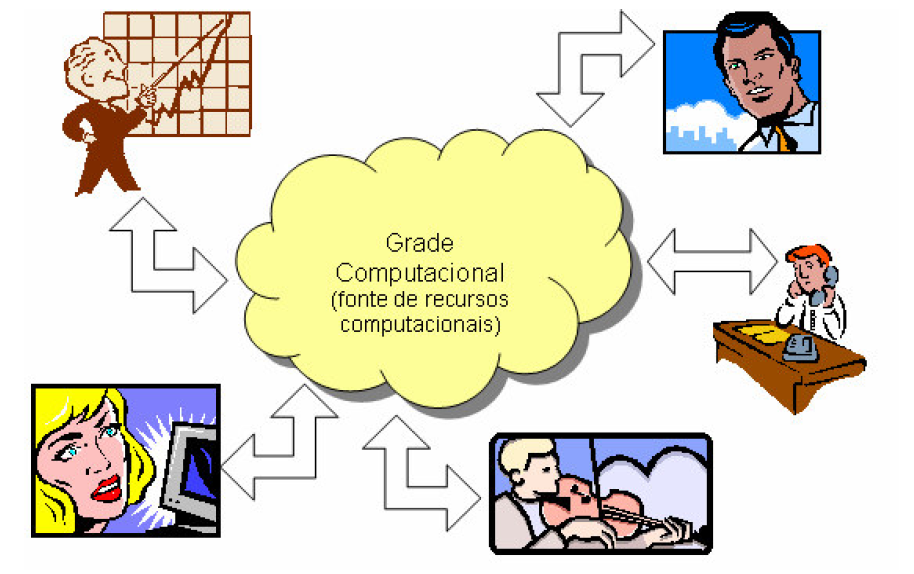
\includegraphics[width=0.6\textwidth]{figuras/grade-comp.png}
	\\\textbf{\footnotesize Fonte: \citeCitacao{cap-livro} }
	\label{fig:figura1}
\end{figure}
\vspace{-0.5cm}

\section{\esp Inserção de tela de software}

Nos casos de telas de \textit{software}, devem ser inseridas como figuras, e referenciadas no texto
como na Figura \ref{fig:tela1}. Além disso, é necessário que seja citada no texto a empresa desenvolvedora.

% Figura
\begin{figure}[!ht]
	\centering	
	\caption[\hspace{0.1cm}Exemplo de tela de software.]{Exemplo de tela de software}
	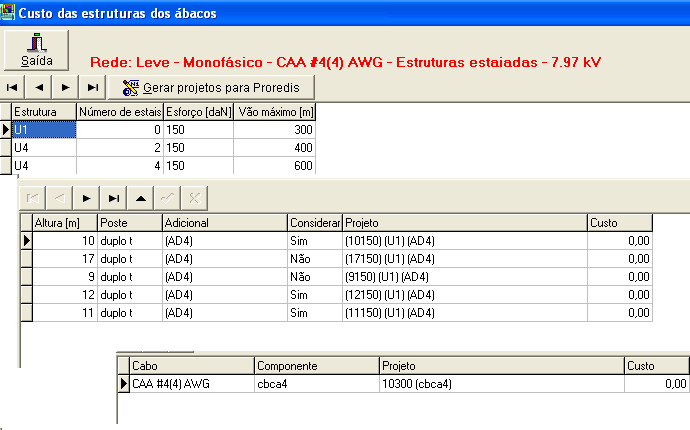
\includegraphics[width=.8\textwidth]{figuras/tela1.png}
	\\\textbf{\footnotesize Fonte: \citeCitacao{tela1}}
	\label{fig:tela1}
\end{figure}

\section{\esp Inserção de gráficos e mapas}

O gráfico é um tipo de ilustração que deve conter todos os elementos citados e também a descrição de seu título
diferenciando-o das figuras da mesma forma que no \ref{gra:grafico1}. 

\begin{grafico}
	\centering	
	\graficos{Exemplo de um gráfico}
	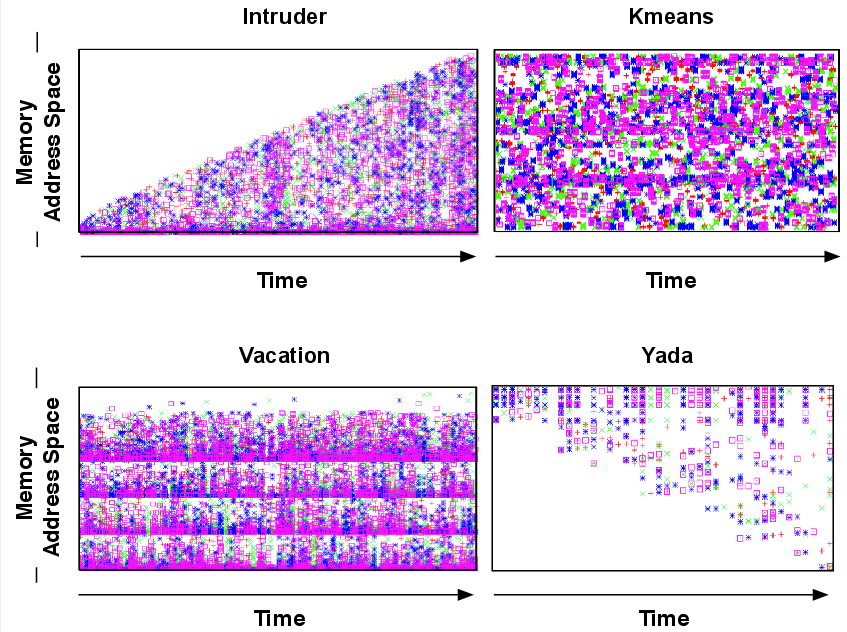
\includegraphics[width=0.7\textwidth]{figuras/access.png}
	\\\textbf{\footnotesize Fonte: \citeCitacao{tese}}
	\label{gra:grafico1}
\end{grafico}

A mesma regra se aplica para mapas, que devem ser adicionados seguindo as regras de apresentação já mostradas. No caso específico,
o título e a numeração, também como os gráficos, devem começar do numeral ``1'' depois da marcação ``Mapa'' seguido do nome do elemento.
Exemplo: \textbf{Mapa 1 - Exemplo de um Mapa}.

 \section{\esp Tabelas}

As tabelas são fechadas nas laterais. Entre os elementos da tabela devem haver linhas. Um exemplo é a Tabela \ref{tab:tabela1}. 

% Tabela
\begin{table}[htb]
	\centering
	\caption{\hspace{0.1cm} Exemplo de uma tabela}
	\vspace{-0.3cm} % espaço entre titulo e tabela
	\label{tab:tabela1}
	% Conteúdo da tabela
	\begin{tabular}{l|c|c}
  \hline
    \textbf{Imagem}	& \textbf{transferência} & \textbf{tempo} \\
    \hline
     estação 1	& 7,72 MB/s &  1:22:18 \\
     estação 2	& 7,72 MB/s &  1:22:17 \\
     estação 3	& 7,59 MB/s & 1:24:25 \\
     estação 4  & 7,53 MB/s & 1:43:27 \\
     estação 5	& 6,14 MB/s  &  1:24:41 \\
     estação 6  &  7,50 MB/s & 1:23:53 \\
     estação 7  & 7,58 MB/s  &  1:24:02 \\
     estação 8  & 7,8 MB/s  &  1:29:06 \\
     estação 9  & 7,9 MB/s  &  1:30:05 \\
     estação 10 & 8,0 MB/s  &  1:32:03 \\
     \hline
 \end{tabular}
	\small
	{\footnotesize\\ \textbf{Fonte: \citeCitacao{monog-fabio}}}
\end{table}

\section{\esp Quadros}

Os quadros diferem das tabelas por apresentarem dados textuais.
Esses dados podem ser esquemáticos, comparativos ou descritivos.

   \begin{quadro}
          \centering
       	\quadros{Bandas/Artistas de Rock e outros}
% 	\vspace{-0.3cm} % espaço entre titulo e tabela
        \label{qua:quadro1}
	\begin{tabular}{|c|c|c|c|} \hline
	\multicolumn{4}{|c|}{\textbf{Bandas ou Artigas de Rock e outros}} 	  \\ 
		\hline \textbf{	Progressivo} & Pink Floyd & Jethro Tull	& Yesterday \\ 
		 \hline \textbf{ Metal}  & Metallica & Iron Maidam & Black Sabath \\ 
		\hline \textbf{	Arena Rock} & Led Zeppelin & The Rolling Stones & Beatles \\ 
		\hline \textbf{ Punk} & Ramones & Black Flag & NOFX	\\ 
		\hline \textbf{	Nacional} & Ira & Engenheiros & Vinil	\\ 
		\hline \textbf{	S.J.E.} & Apolo XI & Invasão 7 & Por do Sol \\ 
		\hline \textbf{	Grunge} & Nirvana & Pear Jam & Alice in Chains	\\ 
		\hline \textbf{	Rock Folk} & Bod Dylan & The Byrds &  The Mamas \& the Papas \\
		\hline \textbf{	Blues} & B.B. King & Albert Colins & Mady Wathers \\ 
		\hline \textbf{	New Wave} & The Police & The Pretenders, &  Duran Duran\\ 
 		\hline \textbf{	Rock Folk} & Bod Dylan & The Byrds &  The Mamas \& the Papas \\
 		\hline \textbf{	Rock alternativo} & R.E.M.& Hüsker Dü & Big Black\\ 
 		\hline
	\end{tabular}
	{\footnotesize\\ \textbf{Fonte: Dados da pesquisa}}
   \end{quadro}

Para gráficos, quadros e tabelas, cujos dados foram extraídos da própria pesquisa, 
 usar a expressão: Dados da pesquisa. Ver exemplo no  \ref{qua:quadro1}.
   

\section{\esp Inserção de algoritmos}

Para inserir um algoritmo, utilizar o exemplo do Algoritmo  \ref{alg:rnagenerica}.
Todos os algoritmos devem ser inseridos como figura, indicada por nome e  fonte. Caso 
forem de própria autoria, isso deverá ser mencionado na fonte, como elaboração feita pelos autores.

\begin{algoritmo}
	\footnotesize
	\algoritmos{Algoritmo genético simples}
	\label{alg:ag}
    \begin{algorithmic}[1]
    		\State Inicialize as probabilidades de cruzamento e mutação, e tamanho da população.
		\State Gere população inicial
		\While{critério convergência não alcançado}
			\State Avalie os indivíduos da população
			\State Execute a seleção
			\State Execute cruzamento
			\State Execute mutação
		\EndWhile{}
  	\end{algorithmic}
	\textbf{\small{Fonte: Adaptado de~\citeCitacao{mestrado}.}}
\end{algoritmo}

Para ilustrações criadas ou adaptadas a partir de outras ilustrações, usar as expressões: 
“Adaptado de...” ou “Criado pelo autor`` com dados extraídos de \ldots
   
   
\chapter{ CITAÇÕES}


Referências deverão ser adicionadas no arquivo \textit{bibliografia.bib}. Cada referência deverá ser adicionada conforme o padrão de normalização da PUC, 
o qual poderá ser consultado na página da biblioteca da PUC Minas \cite{manualpuc}. Todas as publicações citadas no texto deverão ter correspondente nas referências, 
e as indicações de autoria da citação e do ano deverão ser idênticas aos dados expostos.


\section{\esp Citação livre ou indireta}

Quando se reproduzir ideias, sem transcrever as palavras do autor, a indicação da página é opcional. Exemplos desse tipo de citação:
\begin{enumerate} 
 \item [a)] Citação com um autor \cite{knuth}. 
 \item [b)] Citação de artigos em revistas com dois autores \cite{artigo01}.
  \item [c)] Trabalho em congresso com três autores \cite{dovzan:01}.
 \item [d)] Trabalhos com mais de três autores \cite{cap-livro}.
 \item [e)] Dois autores em duas obras distintas \cite{knuth,groupp}.
 \item [d)] Trabalhos distintos com vários autores \cite{congresso,cap-livro}.
 
\end{enumerate}

\section{\esp Citação direta ou textual}

Transcrição literal de textos de outros autores. Nesse caso, deverão ser especificadas as páginas consultadas. 
Se desejar, poderão ser grafadas em itálico para melhor visualização.

\subsection{\esp Textual Curtas}

Quando curtas (até 3 linhas) serão inseridas na sequência normal do texto, entre aspas com as mesma formatação.

\subsection{\esp Textual Longas}

Citações longas (mais de 3 linhas) deverão constituir um parágrafo independente, recuado a 4 cm da margem esquerda, 
com letra tamanho 10 e digitado em espaço simples, sem aspas.
\begin{citacaodireta}
Hegel chama trabalho à forma específica da satisfação das necessidades, que
distingue da natureza o espírito existente. Assim como a linguagem infringe
a imposição da intuição e ordena o caos das múltiplas sensações em coisas
identificáveis, assim o trabalho infringe a imposição do \hspace{0.1cm}desejo \hspace{0.1cm}imediato \hspace{0.1cm}e
suspende, por assim dizer, o processo de satisfação das necessidades.
\cite[25]{habermas}.
\end{citacaodireta}


% Artigo \cite{whatershed:01}

\subsection{\esp Textual de outros idiomas (Tradução)}

\begin{citacaodireta} 
Um \textit{cluster} é um computador paralelo construído de componentes e processos de \textit{software} (tal como sistema de \textit{software}). 
Um \textit{cluster} é formado de nós, cada um contendo um ou mais processadores, memória que é compartilhada por todos os processadores do nodo 
(somente eles), e dispositivos periféricos adicionais (tais como discos), conectados pela rede e que permitem tráfego de dados entre os nós...
\cite[p. 10, tradução nossa]{groupp}\footnote {  … a cluster is a parallel computer that is constructed of commodity  componets and runs 
(as its system software) commodity software. A cluster is made of nodes, each conteining one or more processors, memory that is  shared 
by all of the processors in (and only on) the node, and addtional peripheral devices (surch as disks),
 connected by network that allows data to move between the nodes}.
\end{citacaodireta}
 
\section{\esp Exemplos de citações} 

Alguns exemplos de citações mais utilizadas e/ou que geram algumas dúvidas. É válido observar que não citaremos
todas as possibilidades de citações da norma da PUC Minas, sendo assim é de extrema relevância que se consulte 
o documento no site da Biblioteca da PUC Minas para maiores esclarecimentos acerca de citações \cite{manualpuc}.

\subsection{\esp Citação de monografia, dissertação e tese}

Exemplo de citação de monografia de curso de graduação ou especialização pode ser vista em \citeonline{monog-fabio}.
Exemplo de dissertação de mestrado é referida como \citeonline{mestrado}.

Para o caso de doutorado é citado da seguinte forma, Góes (\citeyear{tese}). Nesse exemplo é válido observar a forma
como está escrito no documento \LaTeX, pois citações que compreendem no texto o nome do autor como sua parte, necessitam 
do parâmetro \verb$\citeonline{}$. 

\subsection{\esp Livros e partes de livros}

Exemplo de capítulo de livro fica conforme este exemplo \cite{cap-livro}.

Para livros citados no corpo do texto e com duas citações juntas, ver os exemplos \citeonline{knuth,groupp}.
Caso essa citação não fizesse parte do texto será referencia dessa forma \cite{knuth,groupp}.

Citações institucionais ou documentos técnicos de alguma entidade devem ser citados desta forma \cite{pmbok}.

\subsection{\esp Tela de software}

Para  citar a tela de um \textit{software} faça da seguinte forma, \citeonline{tela1}.

\subsection{\esp Citações da Biblia Sagrada}

A Bíblia está dividida em duas grandes partes: O Antigo Testamento e o Novo Testamento, divididos em livros, capítulos e versículos. 
Portanto, a citação de partes da Bíblia deve apresentar o título do livro de forma abreviada ou por extenso, o número do capítulo e o número do versículo.


\begin{citacaodireta}
Moisés estendeu a mão sobre o mar. Com um forte \hspace{-0.1cm} vento \hspace{0.1cm} leste a \hspace{0.1cm}sobrar a
noite toda, o Senhor repeliu o mar e o pôs a seco. As águas se fenderam e
os filhos de Israel entraram no meio do mar a pé enxuto, enquanto as águas
formavam uma muralha à direita e à esquerda deles (\citeauthor{biblia} 14,21).
\end{citacaodireta}

\chapter{ CONCLUSÃO}

Discussão dos resultados obtidos na pesquisa. É onde se colocam as observações do autor. 
Poderá também apresentar sugestões de novas linhas de estudo.

A conclusão deve estar de acordo com os objetivos do trabalho.

A conclusão não deve apresentar citações ou interpretações de outros autores.

 \section{\esp Trabalhos futuros}
% 
 Sugestões de estudos posteriores são ser adicionados subseção deste capítulo de conclusão.


%%%%%%%%%%%%%%%%%%%%%%%%%%%%%%%%%%%
%% FIM DO TEXTO
%%%%%%%%%%%%%%%%%%%%%%%%%%%%%%%%%%%

% \selectlanguage{brazil}
%%%%%%%%%%%%%%%%%%%%%%%%%%%%%%%%%%%
%% Inicio bibliografia
%%%%%%%%%%%%%%%%%%%%%%%%%%%%%%%%%%%

 \newpage
 \singlespace{
 \bibliographystyle{abntex2-alf}
 \bibliography{bibliografia}
 }

\end{document}